\begin{frame}[fragile,label=cacheBlockKLoads]{simple blocking -- counting loads}
\lstset{
    style=small,language=C,escapechar=@,
    moredelim=**[is][\btHL<0>]{~2}{~},
    moredelim=**[is][\btHL<0>]{~3}{~},
    moredelim=**[is][\btHL<0>]{~4}{~},
}
\begin{lstlisting}
for (int kk = 0; kk < N; kk += 2)
  for (int i = 0; i < N; i += 2)
    /* load A_i,kk and A_i,kk+1 once into cache in this loop: */
    for (int j = 0; j < N; ++j) {
      /* process a "block" of 2 k values: */
      /* if N large, load Cij and Bkj each iteration: */
      ~2C[i*N+j]~ += ~3A[i*N+kk+0]~ * ~4B[(kk+0)*N+j]~;
      ~2C[i*N+j]~ += ~3A[i*N+kk+1]~ * ~4B[(kk+1)*N+j]~;
    }
\end{lstlisting}
\begin{itemize}
\item (if $N$ large) values from $A_{ik}$ used $N$ times per load
    \begin{itemize}
    \item \myemph<1>{but $A_{i,k}$ and $A_{i,k+1}$ in same cache block: one load for each}
    \end{itemize}
\item (if $N$ large) values from $B_{kj}$ used $1$ times per load
    \begin{itemize}
    \item but good spatial locality, so cache block of $B_{kj}$ together
    \end{itemize}
\item (if $N$ large) values from $C_{ij}$ used \myemph<2>{$2$} times per load
    \begin{itemize}
    \item but good spatial locality, so cache block of $C_{ij}$ together
    \end{itemize}
\end{itemize}
\end{frame}

\begin{frame}{improvement in read misses}
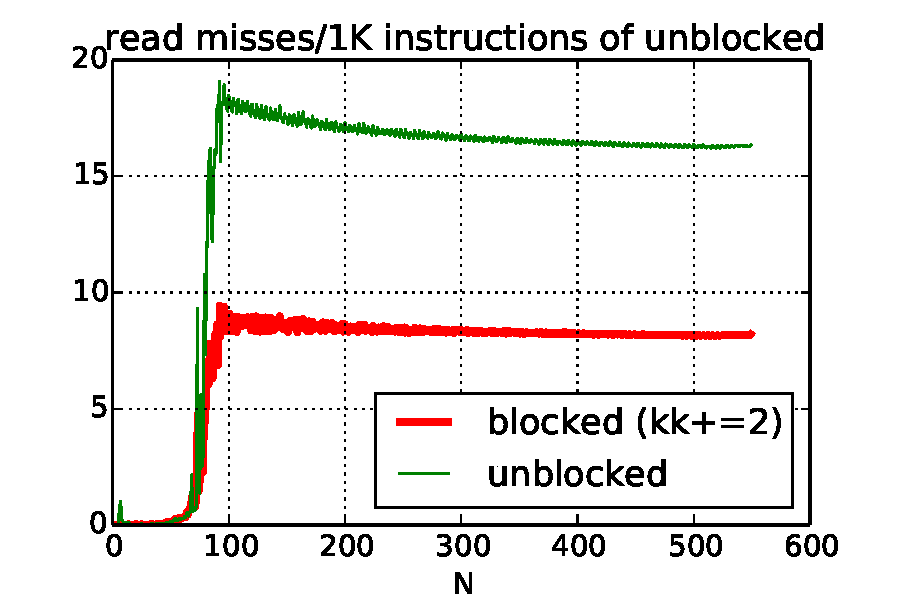
\includegraphics[width=0.8\textwidth]{../caching/k-kk-novec-block-read_miss_rate}
\end{frame}

